\section{Vorbereitungsaufgaben}

\subsection{Energiestruktur eines Atoms}

\subsubsection{Welche Quantenzahlen definieren den Zustand eines Elektrons im Wasserstoffatom?}

Der Zustand des Elektrons im Wasserstoffatom wird definiert durch 4 Quantenzahlen:

-Die Hauptquantenzahl n ,gibt die Schale an,

-die nebenquantenzahl l ,gibt das Unterniveau an,

-die Magnetquantenzahl m ,gibt die Orientierung des Bahndrehimpulses an

und die Spinquantenzahl s. 

\subsubsection{Was ist die Feinstruktur (Spin-Bahn-Kopplung)?}

Die Feinstruktur ist die Aufspaltung der Energieniveaus über die Hauptniveaus hinaus.

\noindent Bei der Spin-Bahn-Kopplung handelt es sich um eine Wechselwirkung zwischen dem Spin und dem eigenen Magnetfeld. Der Gesamtdrehimpuls ergibt sich hierbei aus der Summe des Bahndrehimpulses mit dem Spin.

\subsubsection{Beschreiben sie die LS-Kopplung und die jj-Kopplung.}

Die LS-Kopplung tritt bei leichten Atomen (Ordnungszahl Z<50) auf. Die LS-Kopplung ist die Kopplung zwischen den Bahndrehimpulsen und den Spins der Elektronen. Bei den leichten Atomen ist diese Kopplung stärker als die Spin-Bahn-Kopplung und eine gute Näherung

\noindent Bei schwereren Atomen wird die Spin-Bahn-Kopplung stärker und dann ist die jj-Kopplung eine gute Näherung für die Energiezustände des Atoms. 

\subsection{Magnetisches Moment des Atoms}

\subsubsection{Wie ist der Zusammenhang zwischen dem Magnetischen Moment eines Elektrons und seinen Drehimpulsquantenzahlen?}

Der Zusammenhang ist das gyromagnetische Verhältnis. Dieses beschreibt den Faktor zwischen dem Drehimpuls und dem magnetischen Moment eines Teilchens.

\subsubsection{Was ist der Unterschied zwischen dem gyromagnetischen Verhältnis für den Elektronenspin und demjenigen für den Drehimpuls?}

Das gyromagnetische Verhältnis unterscheidet sich um einen g-Faktor, dieser ist beim Bahndrehimpuls 1 und verändert das Verhältnbis somit nicht. Für den Spin ist dieser g-Faaktor allerdings 2 und deshalb unterscheiden sich die Verhältnisse um einen Faktor 2.

\subsection{Aufspaltung des Energieniveaus eines Atoms im homogenen Feld}

Der Lande Faktor ist das Verhältnis zwischen dem Drehimpuls und dem magnetischen Moment.

\subsubsection{In wie viele Niveaus spaltet sich der Zustand mit Gesamtdrehimpuls J?}

Ein Zustand mit Gesamtdrehimpuls J spaltet sich in 2J+1 äquidistante Niveaus auf.

\subsubsection{Wie ändert sich die Aufspaltung mit der Magnetfeldstärke?}

Bei kleinen Feldstärken tritt der Zeeman Effekt auf. In dieser Auspaltung entstehen äquidistante Energieniveaus und die Spin-Bahn-Kopplung ist vorherrschend.

\noindent Bei grossen Feldstärken ist die LS-Kopplung gestört. Die Energieniveaus sind bei dieser Aufspaltung nicht mehr äquidistant und der Paschen-Bach-Effekt kommt hinzu.

\subsubsection{Was versteht man unter dem Paschen-Bach-Effekt}

Bei grossen Magnetfeldstärken tritt der Paschen-Bach-Effekt auf. Durch die grossen äusseren Magnetfelder wird die LS-Kopplung gestört. Bei der Betrachtung der Spektrallinien sieht der eigentlich auftretende annormale Zeeman Effekt aus wie der normale Zeeman Effekt.

\subsection{Optische Übergänge zwischen Zeemanaufgespaltenen Energieniveaus}

Optische Übergänge sind Übergänge die mit Photonenemission oder -absorption funktionieren. Dabei verändert sich die Magnetquantenzahl m. Erlaubte Übergänge sind Übergänge bei denen gilt, dass die Differenz aus der alten und neuen Quantenzahl m 0, 1 oder -1 ist. Also:

\begin{align}
    m_alt - m_neu = \Delta m = [-1,0,1]
\end{align}

\noindent Es werden bei dem annormalen Zeeman Effekt mehr Spektrallinien beobachtet als beim normalen Zeeman Effekt. Dabei sind die Spektrallinien zirkular polarisiert wenn $\Delta m =  [-1,+1]$ und linear polarisiert, wenn $\Delta m = 0 $.   

\subsection{Optische Übergänge in Cd-Atomen}

\subsubsection{Berechnen sie die Lande Faktoren g\textsubscript{i} und die Aufspaltung $\Delta E$ der Zeeman Linien}

Mit der Formel,

\begin{align}
    g_i = 1 + \frac{j(j + 1) - l(l+1) + s(s+1)}{2j(j+1)}
\end{align}

\noindent wobei j die Gesamtdrehimpulsquantenzahl, l die Bahndrehimpulsquantenzahl und s die Spinquantenzahl ist, lassen sich die Lande Faktoren berechnen.
Für die Zustände $^1p_1$, $^1D_2$, $^3p_1$ und $^3s_1$ ergeben sich folgende Lande Faktoren:

\begin{minipage}{\linewidth}
    \begin{table}[H]
        \centering
    \captionof{table}{Lande Faktoren}
    \begin{tabular}{ll}
        \toprule
        Zustand & Lande Faktor \\
        \midrule
        $^1p_1$ & 1.0 \\
        $^1D_2$ & 1.0 \\
        $^3p_1$ & 1.5 \\
        $^3s_1$ & 2.0 \\
        \bottomrule   
    \end{tabular}
    
    \label{tab:1}
\end{table}
\end{minipage}

\noindent Die Aufspaltung $\Delta E$ wird mit folgender Formel berechnet:

\begin{align}
    \Delta E = (mg_{i,2}-m_1g_{i,1})
\end{align}

\subsection{Dispersionsgebiet und Auflösungsvermögen}

Das Dispersionsgebiet wird mit \ref{dispersion} Formel und das Auflösungsvermögen mit Formel \ref{auflösung} bestimmt. Mit $d = 4 mm$, $L = 120mm$, $n(@644nm) = 1.4567$ und $n(@480nm) = 1.4635$ ergeben sich die Werte in \ref{wdis} und \ref{wauf}.

\begin{equation} \label{dispersion}
    \Delta \lambda_D = \frac{\lambda^2}{2d} \frac{1}{\sqrt{n^2-1}}
\end{equation}

\begin{equation} \label{auflösung}
    A = \frac{L}{\lambda} (n^2-1)
\end{equation}

\begin{align} \label{wdis}
    \Delta \lambda_D(@644) =  48.91pm \\
    \Delta \lambda_D(@480) =  26.95pm 
\end{align}

\begin{align} \label{wauf}
    A_{rot} =  209063.64 \\
    A_{blau} =  285458.06 
\end{align}

\section{Auswertung}

\subsection{Eichung des Elektromagneten}

Für die Eichung des Elektromagneten wird eine Hallsonde verwendet. Diese wird mithilfe eines Stativs zwischen die Polschuhe des Elektromagneten gebracht. Nun wird das Magnetfeld in Abhängigkeit von der Stromstärke gemessen.
Die Ergebnisse dieser Messung sind in \ref{tab:2} zu sehen und noch einmal in \ref{fig:magnet} graphisch dargestellt. Diese graphische Darstellung ist erweitert um eine Ausgleichsrechnung der Form:

\begin{align} \label{B}
    B(I) = a * I^2 + b * I + c.
\end{align}

\noindent Diese lineare Regression wurde mit Python durchgeführt. Dabei entstehen folgende Werte für die Parameter a, b und c:

\begin{align}
    a &= \SI[separate-uncertainty=true]{-5.930(0.325)}{\milli\tesla \per \ampere^2} \\
    b &= \SI[separate-uncertainty=true]{121.318(2.690)}{\milli\tesla \per \ampere}
    c &= \SI[separate-uncertainty=true]{-20.926(4.219)}{\milli\tesla}
\end{align}

\begin{figure}[H]
    \centering
    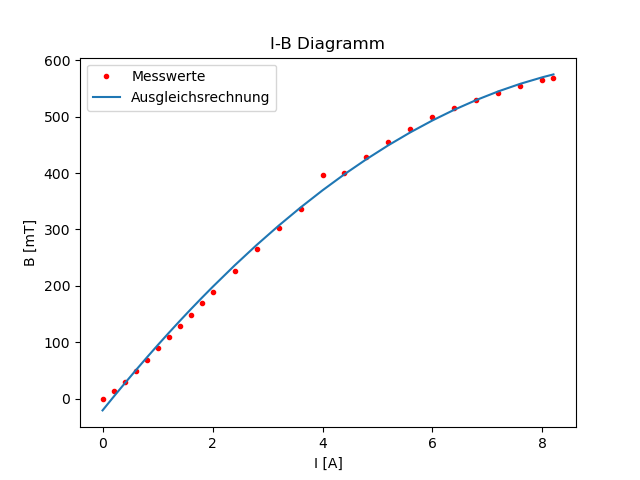
\includegraphics{magnet.png}
    \captionof{figure}{Messwerte der Eichung des Elektromagneten, dargestellt mit dem zugehörigen Ausgleichsgraphen.}
    \label{fig:magnet}
\end{figure}

\subsection{Wellenlängenaufspaltung des Cd-Spektrums}

\subsubsection{Bestimmung des geeigneten Magnetfelds für die Aufnahme der Wellenlängenaufspaltung}

Für die Bestimmung des optimalen Magnetfelds für folgende Messungen ist eine kurze Herleitung der Formel für eben dieses Magnetfeld erforderlich.

\begin{align}
    E &= h \frac{c}{\lambda} \\
    \frac{dE}{D\lambda} &= -h \frac{c}{\lambda^2} \\
    \frac{\Delta E}{\delta \lambda} &= -h \frac{c}{\lambda^2} \\
    \Delta E &= -h \frac{c}{\lambda^2} \delta \lambda \\
    \mu_B g B &= -h \frac{c}{\lambda^2} \delta \lambda \\
    B &= -\frac{hc}{\lambda^2} \delta \lambda \frac{1}{\mu_B g} \\
    B &= -\frac{hc}{\lambda^2} \Delta \lambda_D \frac{1}{\mu_B g} 
\end{align}

\noindent Mit dem planckschen Wirkungsquantum $ h = \SI[separate-uncertainty=true]{6.626e-34}{\joule \second} $, der Lichtgeschwindigkeit $ c = \SI[separate-uncertainty=true]{3e8}{\metre \per \second} $ und dem Bohrschen Magneton $ \SI[separate-uncertainty=true]{9.274e-24}{\joule\per\tesla} $ ergeben sich für das optimale Magnetfeld die Werte in \ref{tab:3}.

\begin{minipage}{\linewidth}
    \begin{table}[H]
        \centering
    \captionof{table}{optimale Magnetfeldstärken}
    \begin{tabular}{lll}
        \toprule
        Farbe & Polarisation & optimale B-Feldstärke [T] \\
        \midrule
        Rot & $ \sigma $ & 0.632 \\
        Blau & $ \pi $ & 1.253 \\
             & $ \sigma $ & 0.418 (g=$ \frac{3}{2} $)\\
             & $ \sigma $ & 0.313 (g=2)\\
        \bottomrule   
    \end{tabular}
    
    \label{tab:3}
\end{table}
\end{minipage}

\subsection{Wellenlängenaufspaltung der roten Linie}

\noindent Um die Wellenlängenaufspaltung zu bestimmen, werden die aufgenommenen Bilder \ref{fig:rotohne} und \ref{fig:rotmit} mit Paint analysiert. Dabei wird jeweils der Abstand zwischen den Spektrallinien in Pixeln betrachtet und dann mittels Formel \ref{welle} in die Wellenlängenaufspaltung umgerechnet. Bei der Rechnung wurde davon ausgegangen, dass der Abstand mit einer ungenauigkeit von 5 Pixeln bestimmt wurde. Mit dieser Unsicherheit wurde mittels Python eine Fehlerrechnung durchgeführt und die resultierende Unsicherheit ist, genau wie der Wert der Aufspaltung, in Tabelle \ref{tab:Wellerot} zu sehen.

\begin{equation}
    \delta \lambda = \frac{1}{2} \frac{\delta s}{\Delta s} \Delta \lambda_D \label{welle}
\end{equation}

\noindent Um nun die Energiedifferenz und den Lande-Faktor zu bestimmen muss zunächst das Magnetfeld bestimmt werden. Es wurde mit einer Stromstärke von $ \SI{7.8}{\ampere} $ ein Magnetfeld erzeugt bei dieser Messung. Nach \ref{B} ist das ein Magnetfeld von $\SI{564.5732}{\milli\tesla}$.
Die Energiedifferenz $ \Delta E $ lässt sich mit 

\begin{equation} \label{dE}
    \Delta E = \frac{h * c}{\lambda^2} * \delta \lambda
\end{equation}

\noindent bestimmen. Dabei ist h das Plancksche Wirkungsquantum, c die Lichtgeschwindigkeit, $ \lambda $ die Wellenlänge und $ \delta \lambda $ die Wellenlängenänderung. Mit dem Bohrschen Magneton und Gleichung \ref{Lande} lässt sich nun der Lande Faktor bestimmen. 

\begin{equation} \label{Lande}
    g_{ij} = \frac{\Delta E}{B * \mu_B} 
\end{equation}

\noindent Werden in diese Gleichungen nun alle Werte eingetragen so entstehen diese Ergebnisse:

\begin{align*}
    B &= \SI{564.573}{\milli\tesla} \\
    \Delta E &= \SI{3.106e-24}{\joule} \\
    g_{ij} &= 0.593 
\end{align*}

\subsection{Zeemanaufspaltung der blauen Linie}

Das Vorgehen bei der Auswertung der Bilder für die blaue Spektrallinie verläuft analog. Diesmal werden die Bilder \ref{fig:blauohne} und \ref{fig:blausigma} verwendet. Diese werden auch mit der Formel \ref{welle} in die Wellenlängenaufspaltung umgerechnet. Die Fehlerrechnung verläuft analog. Die den Bildern entnommenen Werte und die entstehenden Werte sind in \ref{tab:Welleblau} zu sehen.

\noindent Auch für die Berechnung des Lande Faktors für die blaue Linie wird die gleiche Rechnung verwendet. Es werden die Gleichungen \ref{B}, \ref{dE} und \ref{Lande} verwendet. Dabei entstehen folgende Werte:

\begin{align*}
    B &= \SI{369.466}{\milli\tesla} \\
    \Delta E &= \SI{5.686e-24}{\joule} \\
    g_{ij} &= 1.660 
\end{align*}

\section{Diskussion}

\subsection{Allgemeine Fehlerquellen bei der Durchführung und dem Aufbau}

Bei der Durchführung dieses Versuchs sind einige Fehlerquellen entstanden. Das Magnetfeld lies sich für eine auswertbare Aufnahme von Bildern der blauen pi-Linie überhaupt nicht einstellen. Das Ergebnis ist \ref{fig:blaupi}. Dieses Bild lies sich nicht schärfer einstellen und so können keine Werte abgelesen werden. 

\noindent Weiterhin ist die Feinjustierung des Aufbaus sehr komplex und kleine Veränderungen erzeugen ein stark verändertes Bild. 

\noindent Ausserdem war es nicht möglich noch mehr Ordnungen der einzelnen Aufspaltungen scharf ins Bild zu bekommen. Daher entsteht ein grösserer Fehler, weil der Mittelwert aus weniger Werten zusammengesetzt ist. 

\noindent Die Eichung des Magnetfelds ist auch fehlerbehaftet, da diese von mit dem Auge abgelesenen Werten und einer fehlerbehafteten Ausgleichsrechnung abhängt.

\noindent Auch die anschliessende Auswertung der Bilder liefert Fehlerquellen. Bei dem ablesen des Pixelabstands musste mit dem Auge das Zentrum der einzelnen Linien bestimmt und dann mit der Maus anvisiert werden. Auch hierbei werden Ungenauigkeiten entstanden sein. 

\subsection{Abweichung der Werte}

Die berechneten Werte sowie die zugehörigen Literaturwerte und die Abweichungen der berechneten zu den Literaturwerten sind in \ref{tab:Lande} eingetragen. Es ist zu erkennen, dass der Wert für die blaue $\sigma$-Linie deutlich näher am Literaturwert liegt als der für die rote Linie. Dies war nach der Durchführung auch so zu erwarten. Während die blaue $\sigma$-Linie verhältnismässig einfach scharf abzulichten war, bereitete die rote $\sigma$-Linie an der Stelle grössere Schwierigkeiten. Dort hat es sehr viel Arbeit gebraucht um mehrere Ordnungen scharf ins Bild zu bekommen und trotz mehrfacher Feinjustierung sind es immer noch weniger Ordnungen als bei der blauen Linie. Der Messwert der blauen Linie profitiert daher von mehr Messwerten, da mehr Ordnungen abzulesen sind. 
Dabei war das Magnetfeld ein grosses Hindernis. Denn neben allen anderen bereits erwähnten Fehlerquellen, lässt sich auch für die rote Linie das Magnetfeld nicht hoch genug einstellen. Das Problem gab es bei der blauen $\sigma$-Linie nicht. Unter Berücksichtigung all dieser Fehlerquellen und durch den Aufbau bedingten Probleme haben die Werte allerdings keine Abweichung, die sich nicht durch diese erklären lässt. Das Experiment ist also als erfolgreich durchgeführt einzustufen. 

\begin{minipage}{\linewidth}
    \begin{table}[H]
        \centering
    \captionof{table}{Berechnete Lande Faktoren und die Abweichung}
    \begin{tabular}{llll}
        \toprule
        Farbe & Berechneter Lande Faktor & Literatur Lande Faktor & Abweichung \\
        \midrule
        Blau & 1.660 & 1.75 & 5.14\% \\
        Rot & 0.593 & 1 & 40.7\% \\
        \bottomrule   
    \end{tabular}
    
    \label{tab:Lande}
\end{table}
\end{minipage}

\section{Literatur}

\url{https://moodle.tu-dortmund.de/pluginfile.php/1929918/mod_resource/content/5/V27-Mai2019.pdf}

\noindent \url{https://de.wikipedia.org/wiki/Bohrsches_Magneton}

\noindent \url{https://de.wikipedia.org/wiki/Plancksches_Wirkungsquantum}

\section{Messwerte}

\begin{minipage}{\linewidth}
    \begin{table}[H]
        \centering
    \captionof{table}{Messreiehe zur Eichung des Elektromagneten}
    \begin{tabular}{ll}
        \toprule
        Zustand & Lande Faktor \\
        \midrule
        0   & 0 \\
        0.2 & 14 \\
        0.4 & 30 \\
        0.6 & 49 \\
        0.8 & 68 \\
        1   & 90 \\
        1.2 & 109 \\
        1.4 & 129 \\
        1.6 & 149 \\
        1.8 & 169 \\
        2   & 190 \\
        2.4 & 227 \\
        2.8 & 266 \\
        3.2 & 302 \\
        3.6 & 336 \\
        4   & 396 \\
        4.4 & 400 \\
        4.8 & 429 \\
        5.2 & 455 \\
        5.6 & 479 \\
        6   & 500 \\
        6.4 & 516 \\
        6.8 & 530 \\
        7.2 & 543 \\
        7.6 & 555 \\
        8.0 & 566 \\
        8.2 & 569 \\
        \bottomrule   
    \end{tabular}
    
    \label{tab:2}
\end{table}
\end{minipage}

\begin{minipage}{\linewidth}
    \begin{table}[H]
        \centering
    \captionof{table}{Wellenlängenaufspaltung der roten Linie}
    \begin{tabular}{llll}
        \toprule
        Ordnung & $ \Delta s $ [px] & $ \delta s $ [px] & $ \delta \lambda $ \\
        \midrule
        1 & 365 & 110 &  $ \SI[separate-uncertainty=true]{7.375(0.350)}{e-12\metre} $ \\
        2 & 290 & 72  &  $ \SI[separate-uncertainty=true]{6.498(0.437)}{e-12\metre} $ \\
        3 & 245 & 60  &  $ \SI[separate-uncertainty=true]{5.993(0.514)}{e-12\metre} $ \\
        4 & 220 & 55  &  $ \SI[separate-uncertainty=true]{6.118(0.573)}{e-12\metre} $ \\
        5 & 190 & 50  &  $ \SI[separate-uncertainty=true]{6.440(0.666)}{e-12\metre} $ \\
        \midrule
        Mittelwert & & & $ \SI[separate-uncertainty=true]{6.48(0.23)}{e-12\metre} $ \\
        \bottomrule   
    \end{tabular}
    
    \label{tab:Wellerot}
\end{table}
\end{minipage}

\begin{minipage}{\linewidth}
    \begin{table}[H]
        \centering
    \captionof{table}{Wellenlängenaufspaltung der blauen Linie}
    \begin{tabular}{llll}
        \toprule
        Ordnung & $ \Delta s $ [px] & $ \delta s $ [px] & $ \delta \lambda $ \\
        \midrule
        1 & 275 & 150 &  $ \SI[separate-uncertainty=true]{7.351(0.279)}{e-12\metre} $ \\
        2 & 220 & 115  &  $ \SI[separate-uncertainty=true]{7.044(0.346)}{e-12\metre} $ \\
        3 & 190 & 105  &  $ \SI[separate-uncertainty=true]{6.545(0.428)}{e-12\metre} $ \\
        4 & 175 & 85  &  $ \SI[separate-uncertainty=true]{7.447(0.405)}{e-12\metre} $ \\
        5 & 160 & 75  &  $ \SI[separate-uncertainty=true]{5.896(0.460)}{e-12\metre} $ \\
        6 & 150 & 70  &  $ \SI[separate-uncertainty=true]{5.840(0.490)}{e-12\metre} $ \\
        7 & 135 & 60  &  $ \SI[separate-uncertainty=true]{5.989(0.546)}{e-12\metre} $ \\
        \midrule
        Mittelwert & & & $ \SI[separate-uncertainty=true]{6.59(0.16)}{e-12\metre} $ \\
        \bottomrule   
    \end{tabular}
    
    \label{tab:Welleblau}
\end{table}
\end{minipage}

\begin{figure}[H]
    \centering
    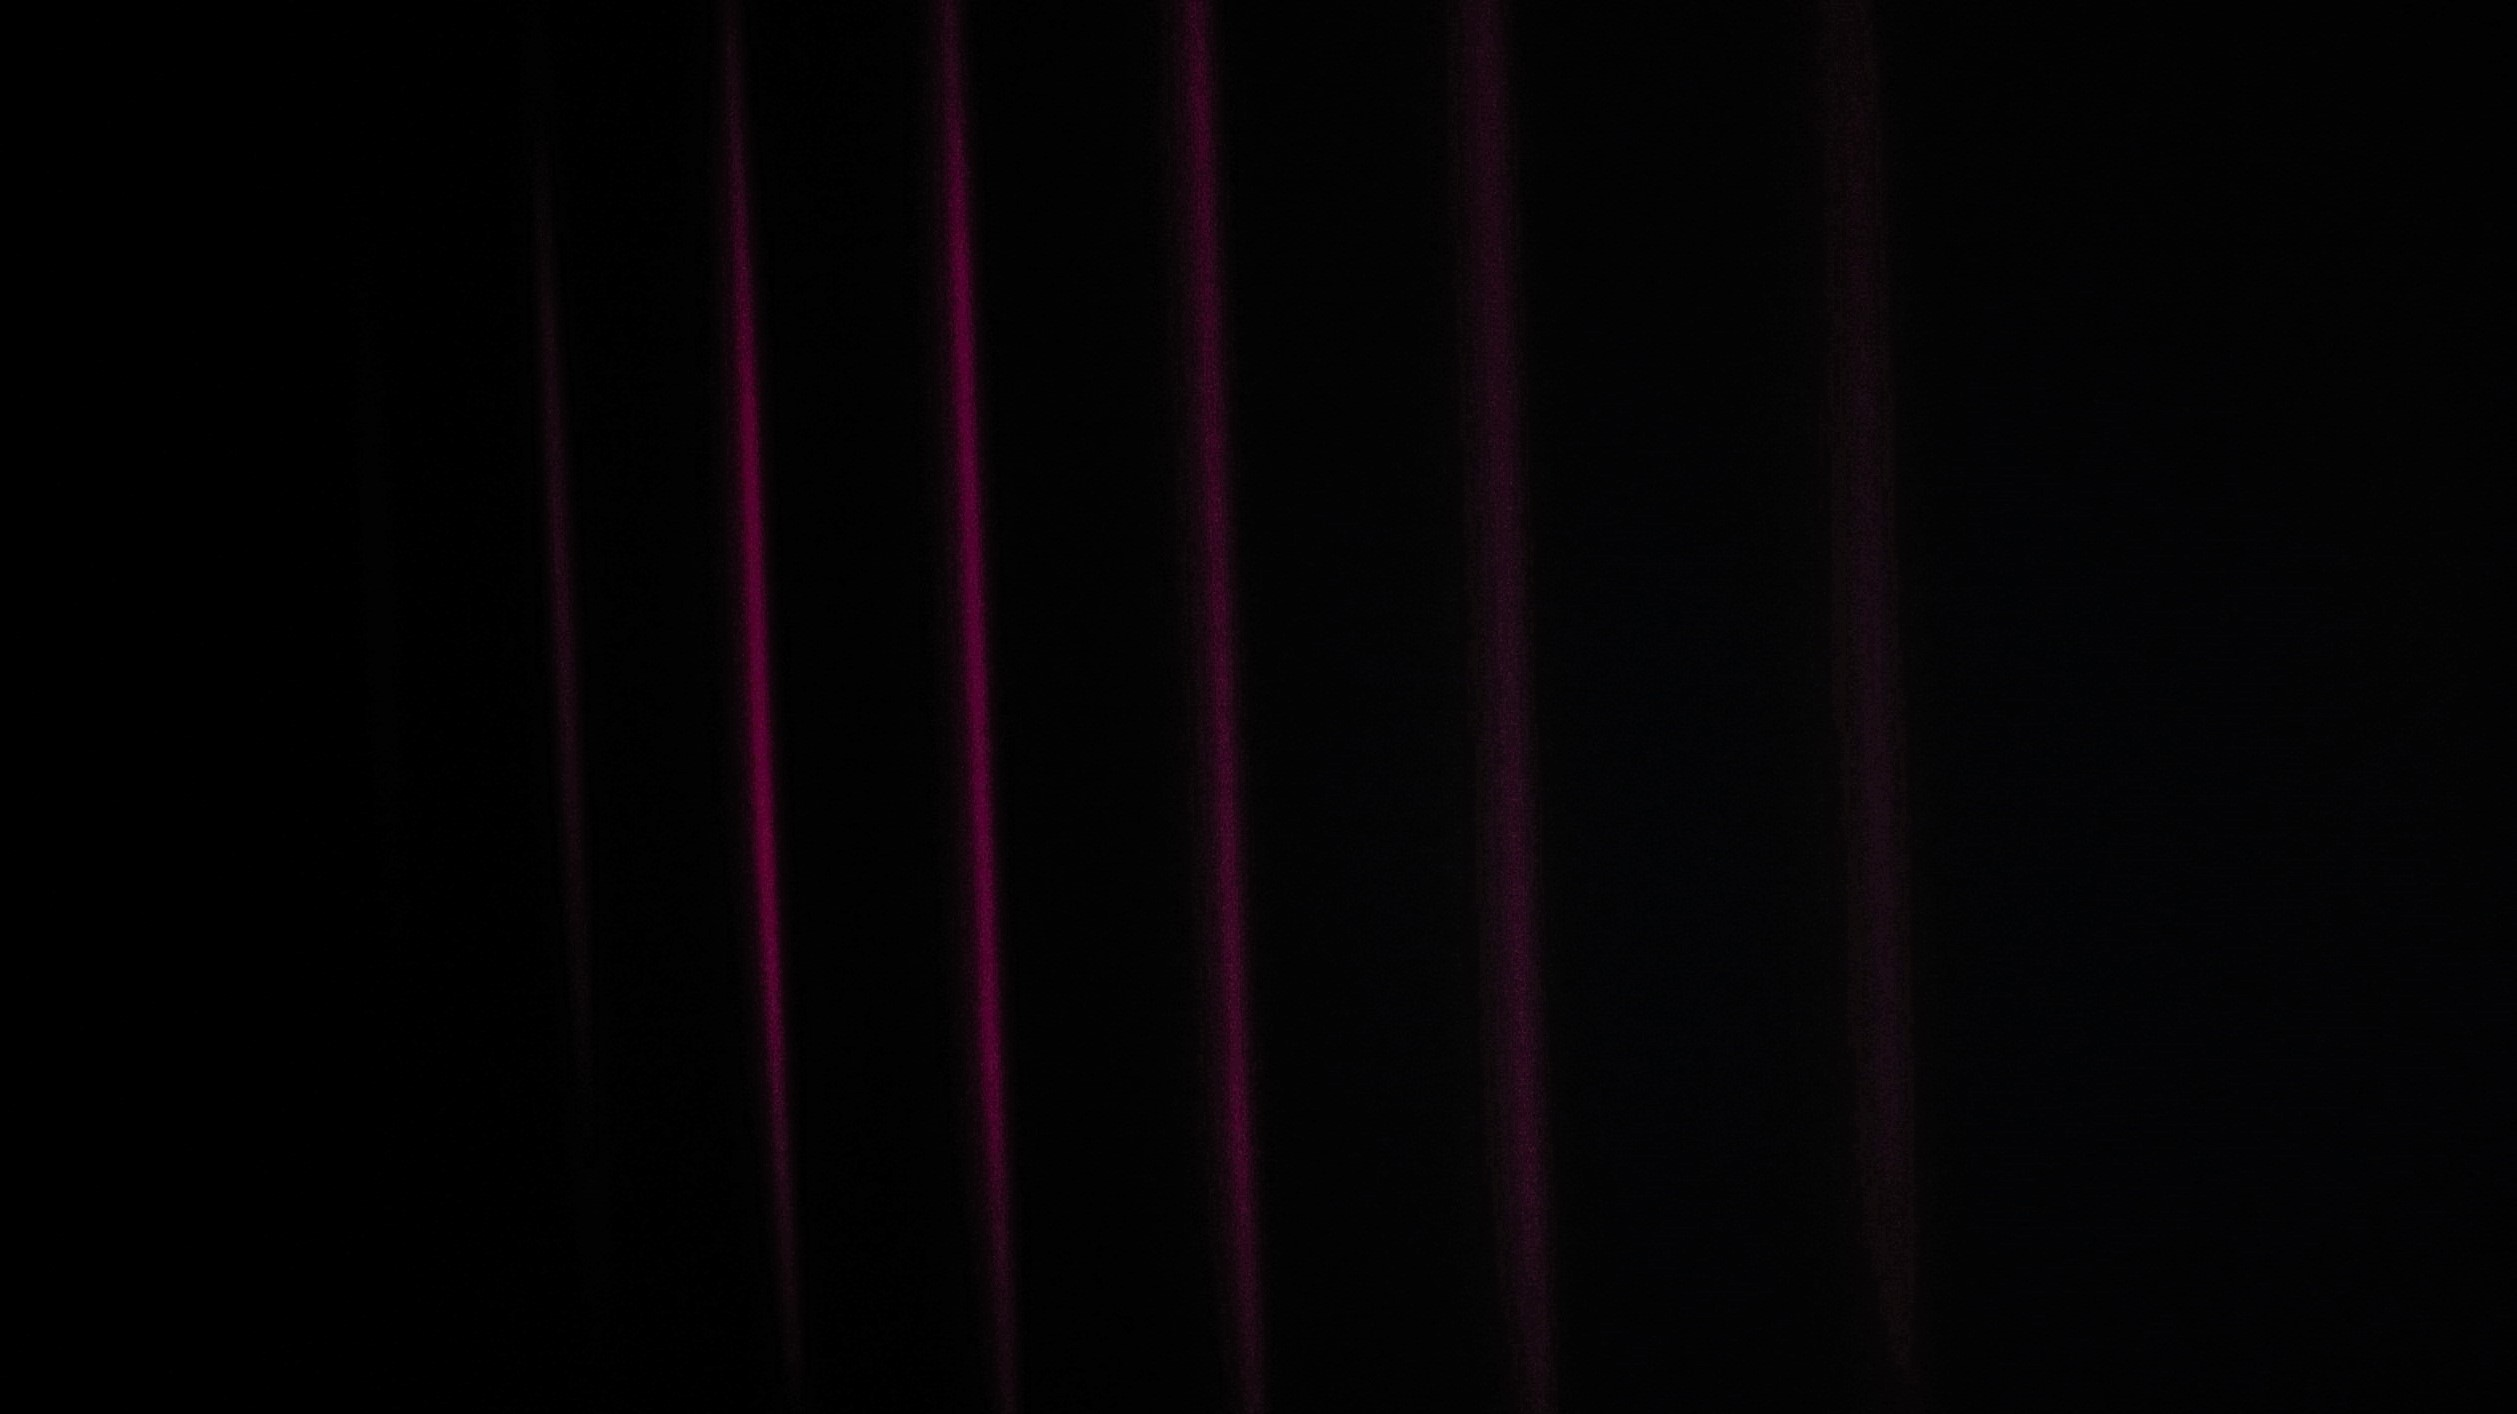
\includegraphics[scale=0.4]{rotohne3.jpg}
    \captionof{figure}{Wellenlängenaufspaltung der roten Linie ohne B-Feld.}
    \label{fig:rotohne}
\end{figure}

\begin{figure}[H]
    \centering
    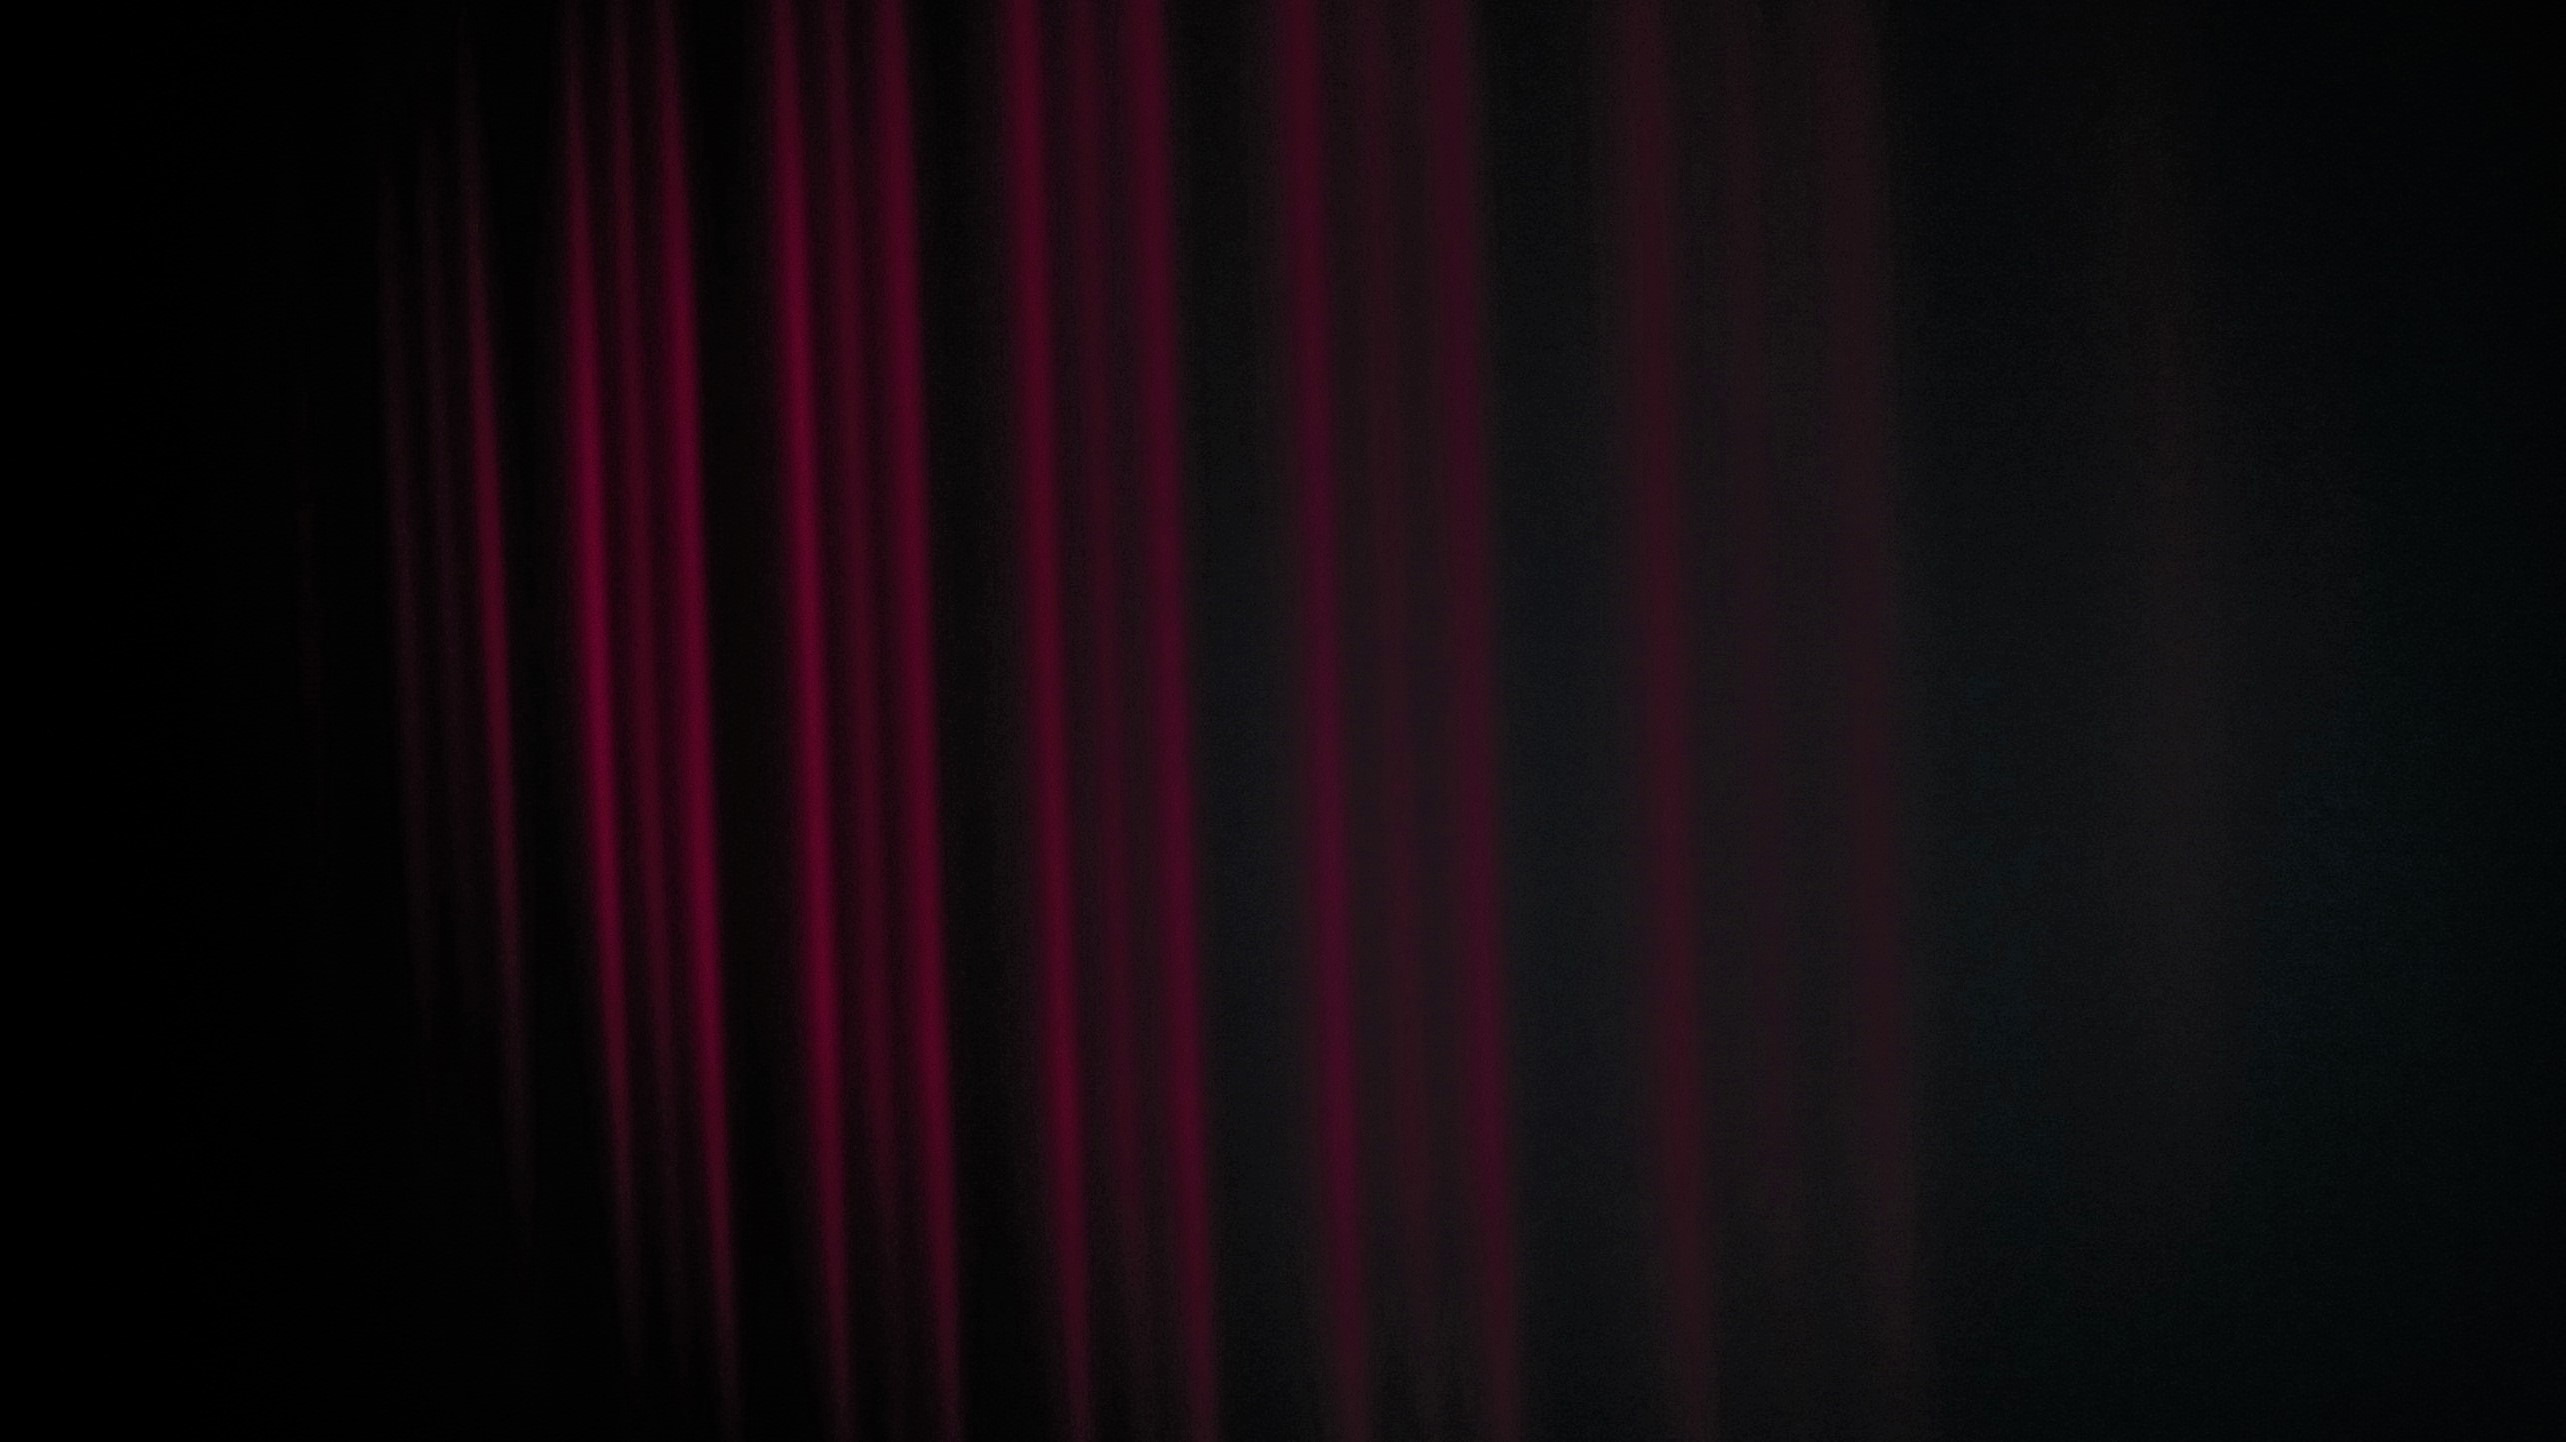
\includegraphics[scale=0.4]{rotmit2.jpg}
    \captionof{figure}{Wellenlängenaufspaltung der roten Linie mit B-Feld.}
    \label{fig:rotmit}
\end{figure}

\begin{figure}[H]
    \centering
    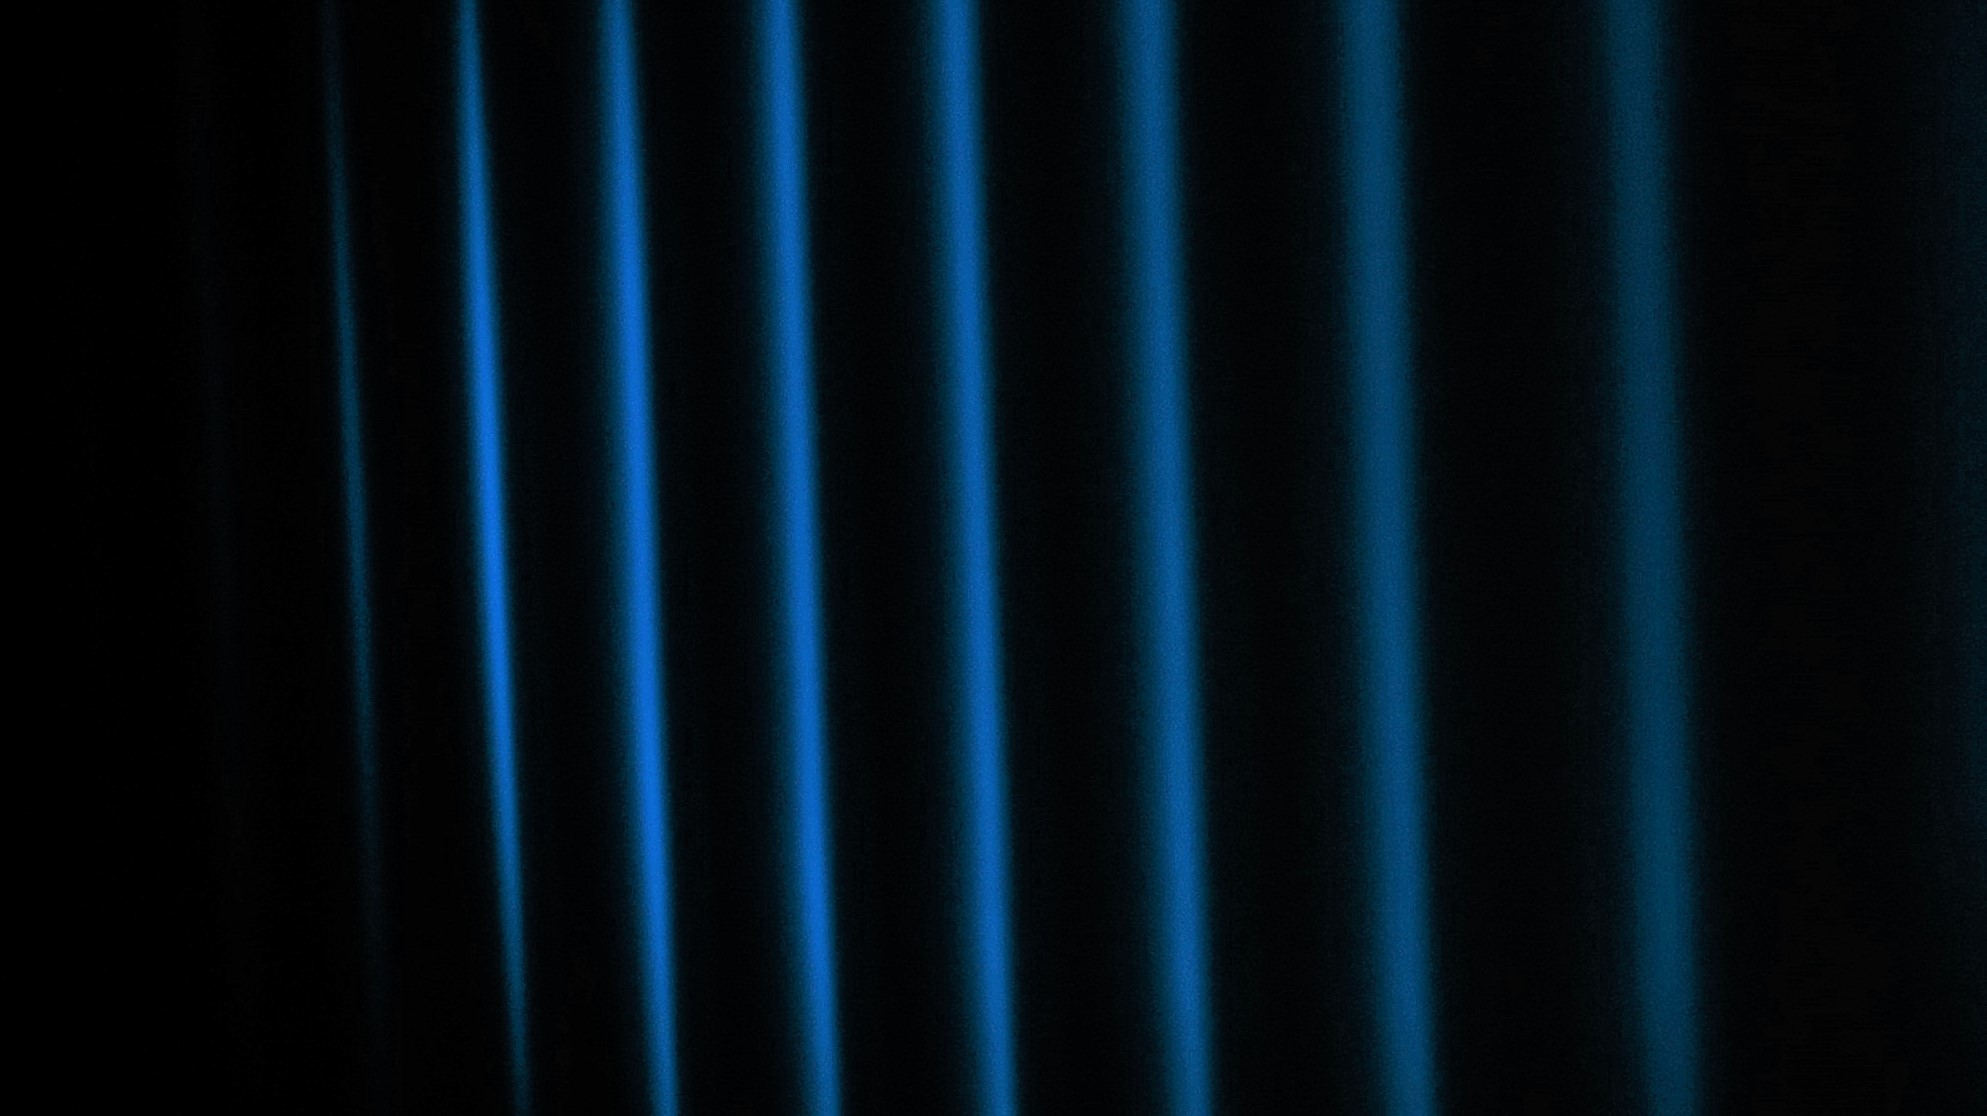
\includegraphics[scale=0.4]{blauohne.jpg}
    \captionof{figure}{Wellenlängenaufspaltung der blauen Linie ohne B-Feld.}
    \label{fig:blauohne}
\end{figure}

\begin{figure}[H]
    \centering
    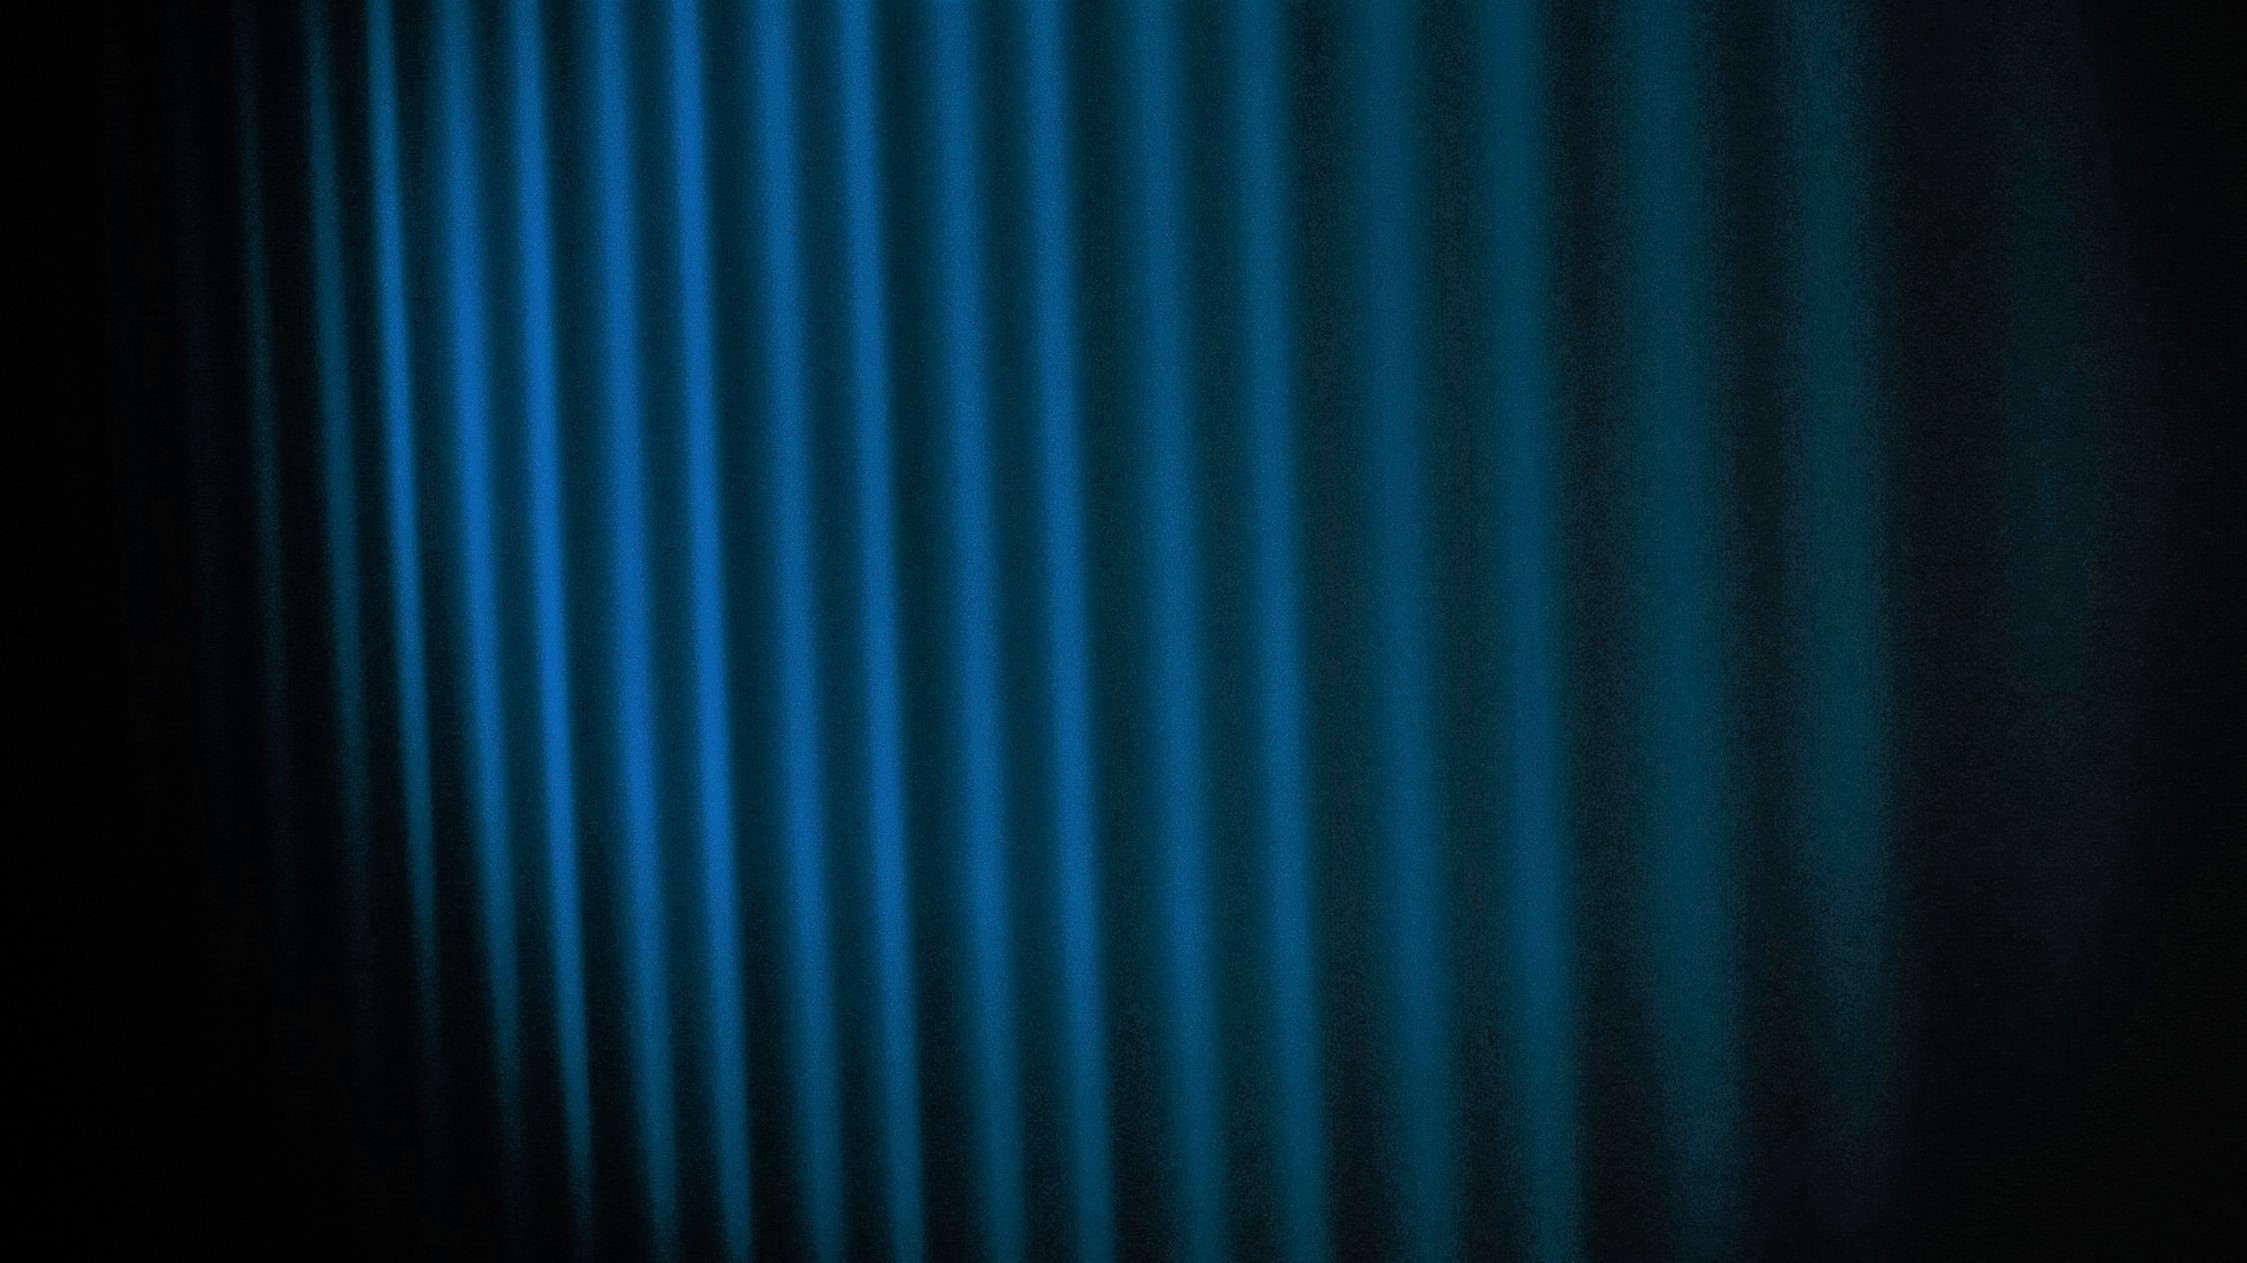
\includegraphics[scale=0.4]{blausigma.jpg}
    \captionof{figure}{Wellenlängenaufspaltung der blauen $\pi$-Linie ohne B-Feld.}
    \label{fig:blausigma}
\end{figure}

\begin{figure}[H]
    \centering
    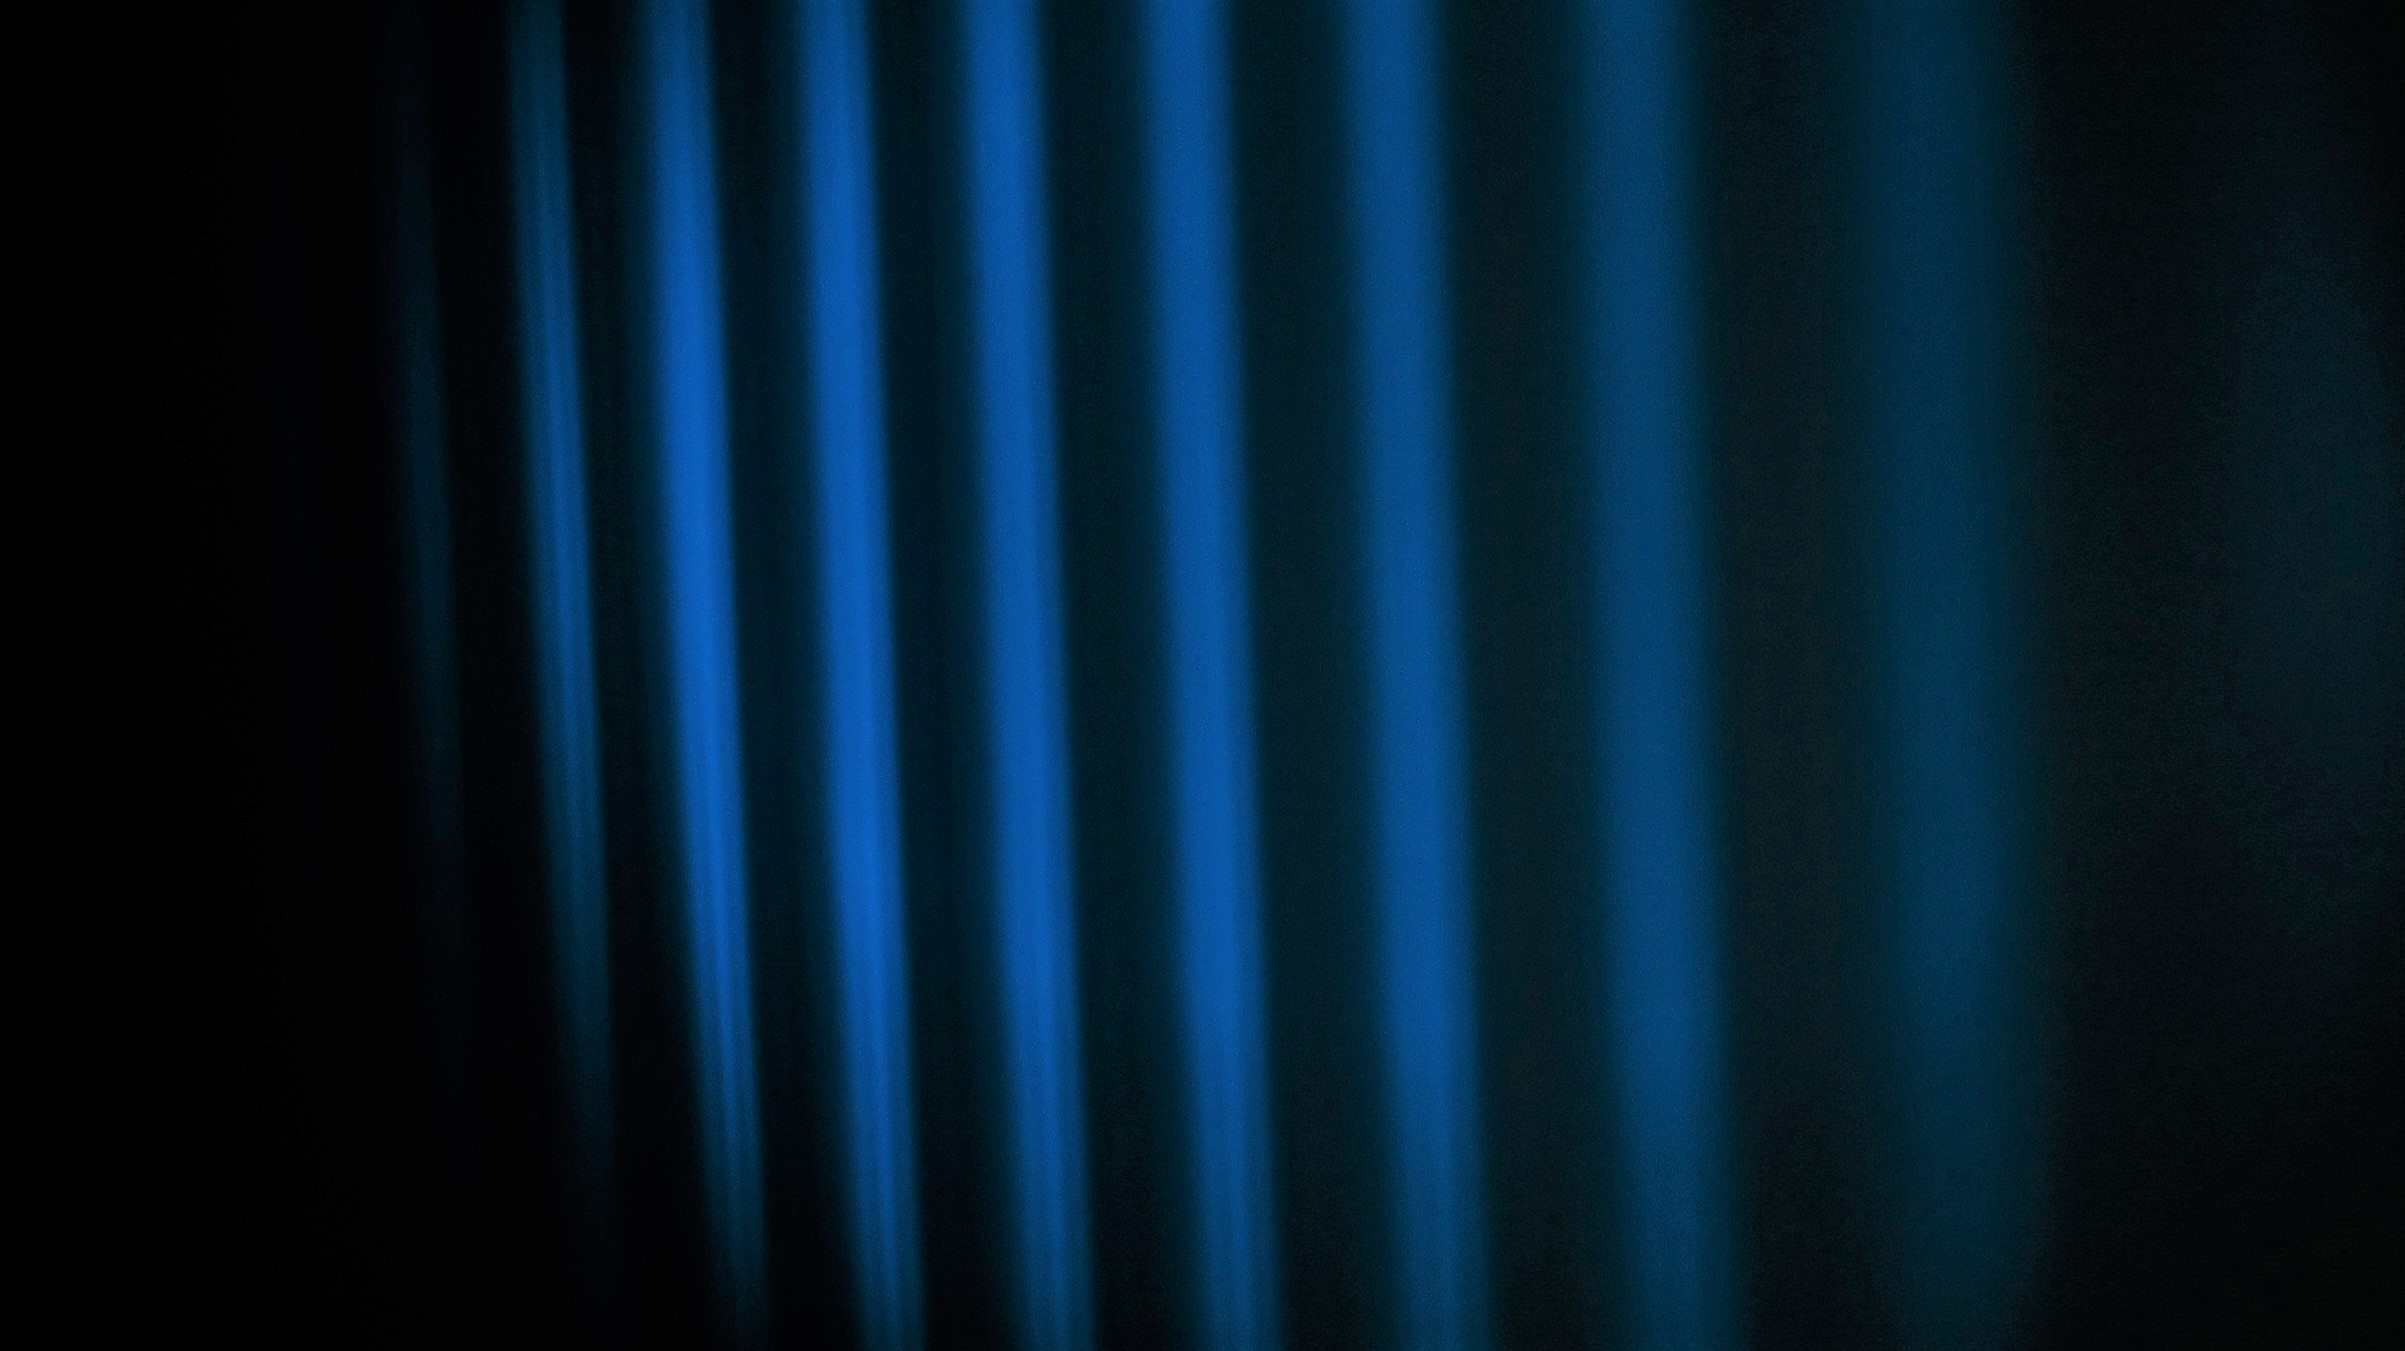
\includegraphics[scale=0.4]{blaupi.jpg}
    \captionof{figure}{Wellenlängenaufspaltung der blauen $\sigma$-Linie ohne B-Feld.}
    \label{fig:blaupi}
\end{figure}